
\documentclass[letterpaper,oneside]{book}%


\usepackage[left=1in,right=1in,top=1in,bottom=1in]{geometry}

\usepackage{amsmath}
\usepackage{amssymb}
\usepackage{amsthm}
\usepackage{amsfonts}
\usepackage{tikz}
\usepackage{graphicx}

\newcommand{\ds}{\displaystyle}
\newcommand{\dfdx}[1]{\frac{d#1}{dx}}
\newcommand{\ddx}{\frac{d}{dx}}


\usepackage{color}
\definecolor{darkblue}{rgb}{0, 0, .6}
\usepackage[breaklinks]{hyperref}
\hypersetup{
	colorlinks=true,
	linkcolor=darkblue,
	anchorcolor=darkblue,
	citecolor=darkblue,
	pagecolor=darkblue,
	urlcolor=darkblue,
}

\begin{document}
\noindent {\large Mars Rover - Contour Plots, Surface Plots, and Gradient Fields - Local Optimization}

\hrule
\vspace{.2in} 

The map below is a topographical map of a location at Crater's of the Moon National Park. The grid was added over the top of the map, and distances were adjusted to make some computations below simpler.  
\begin{center}
  \begin{tikzpicture}[scale=1.91]
    \node at (4,3){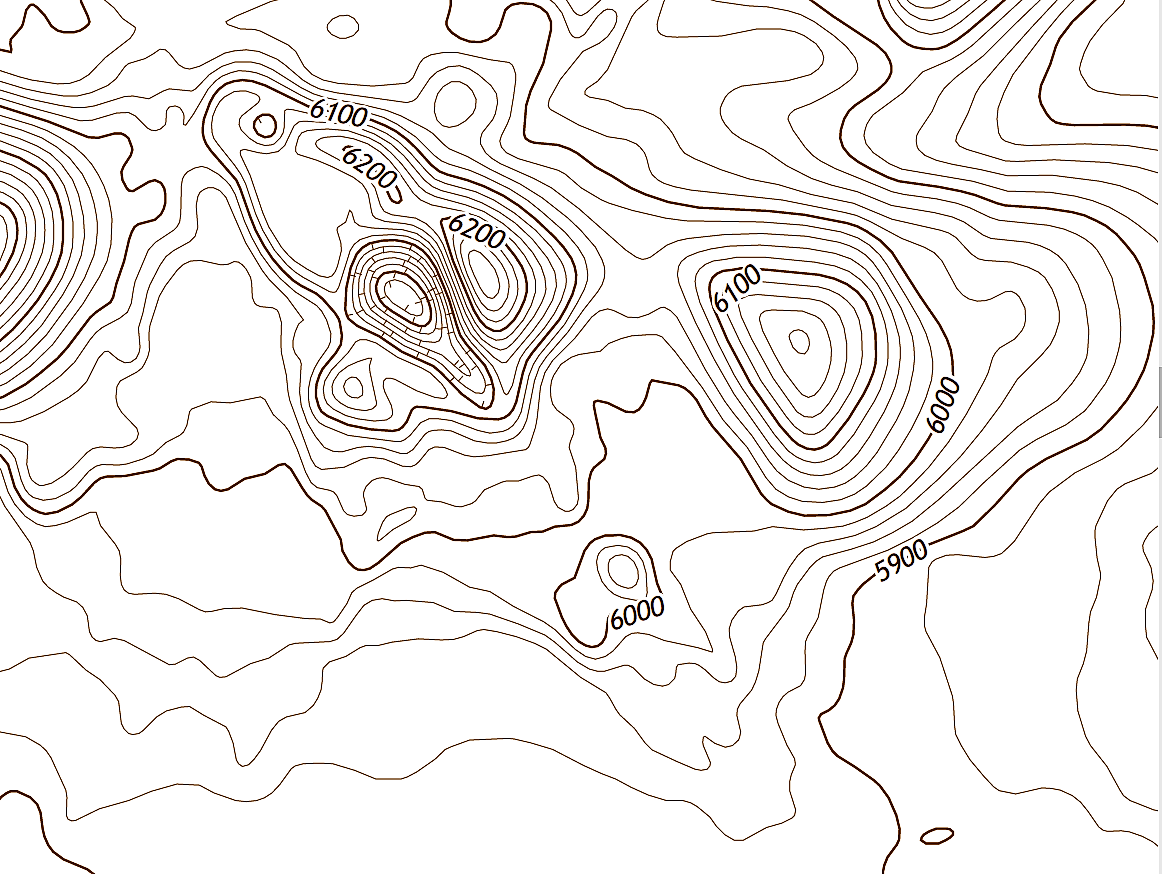
\includegraphics[width=6in]{pseudoMarsTopo.png}};
    \draw[thin,gray] (0,0) grid (8,6);
    \draw[->,thick] (0,0) -- (8,0)node[below]{$x$ (1000 ft)};
    \draw[->,thick] (0,0) -- (0,6)node[above]{$y$ (1000 ft)};
    \node at (-.15,1) {1};
    \node at (-.15,2) {2};
    \node at (-.15,3) {3};
    \node at (-.15,4) {4};
    \node at (-.15,5) {5};
    \node at (1,-.15) {1};
    \node at (2,-.15) {2};
    \node at (3,-.15) {3};
    \node at (4,-.15) {4};
    \node at (5,-.15) {5};
    \node at (6,-.15) {6};
    \node at (7,-.15) {7};
    \filldraw (1,2) circle (1pt) node[above right]{$A$}; 
    \filldraw (5,5) circle (1pt) node[above right]{$B$}; 
    \filldraw (7,4.58) circle (1pt) node[above right]{$C$}; 
    \filldraw (.45,4.4) circle (1pt) node[left]{$D$}; 
    \filldraw (6,2) circle (1pt) node[below right]{$E$}; 
\end{tikzpicture}
\end{center}
The contours on the map represent a function $z=f(x,y)$, where $z$ is the elevation in meters, with contours drawn at 20 ft increments.  We've added a 1000 ft grid over the map to aid in navigation. Suppose a hiker is currently at $A$. The hiker wants to get to $B$. Discuss the answers to each question below with your group.

\begin{enumerate}
 \item What is the elevation 2000 ft east and 3000 ft north, so at $(2,3)$? In other words give $f(2,3)$.  
 \item Note that $A=(1,2)$. Estimate $f(A)$. Then estimate each of $f(B)$,   $f(C)$,   $f(D)$, and $f(E)$.
 \item On the map, are there any hill tops (local maximums)?  Where are they? 
 \item Mark the spot on the map with the highest elevation. [Hint: it is not on a hill top.]
 \item How do you locate local minimums (low points)? Mark them.
 \item On the map, where are the steepest inclines? Where are the mostly flat bits of land?
 \item Why is a straight path from $A$ to $B$ not a good idea?
 \item If you followed a straight path from $A$ to $B$, where is the steepest slope encountered? 
 \item Plan a route to get from point $A$ to point $B$ that passes through one other point (call it $F$), with straight lines connecting $A$ and $B$ to $F$, avoiding steep rises and falls. Draw this route on your map. 
 \item There are three other points on the map ($C$, $D$, and $E$).  At each of these points, we'll estimate the slope of the hill in two different directions, namely moving east or north, and then use these estimates to construct a vector, called the gradient, that we can use to help us navigate. 
 \begin{enumerate}
  \item At point $C$, notice that moving right $\Delta x \approx 100$ m (so 0.1 km) doesn't really change the elevation much at all (maybe there is a slight drop, but very small). This suggests that $\Delta z\approx 0$ and so the slope when moving east is $\ds\dfrac{\Delta z}{\Delta x}\approx\frac{0}{100}=0$. 
  \item At point $C$, moving north about $\Delta y = 100$ m gets us to the next contour, which is a drop of $\Delta z \approx -20$ m.  This gives a slope of $\ds\dfrac{\Delta z}{\Delta y} \approx \frac{-20}{100} = -0.2$, a 20\% downhill grade. 
  \item Above we estimated $\ds\dfrac{\Delta z}{\Delta x}\approx\frac{0}{100}=0$ and $\ds\dfrac{\Delta z}{\Delta y} \approx \frac{-20}{100} = -0.2$. We can draw an arrow starting from point $C$ that moves right 0 units and up $-0.2$ units (so the arrow points straight down). This vector we call the gradient of $f$ at $C$ and write it symbolically as $$\vec \nabla f(C) = \left<0,-0.2\right> = 0{\bf i}-0.2{\bf j} = 0\vec i-0.2\vec j.$$
  \item  Estimate $\dfrac{\Delta z}{\Delta x}$ at point $D$. 
  \item  Estimate $\dfrac{\Delta z}{\Delta y}$ at point $D$. 
  \item  Draw an arrow starting at $D$ that moves right $\dfrac{\Delta z}{\Delta x}$ units and up $\dfrac{\Delta z}{\Delta y}$ units, in other words draw the gradient of $f$ at $D$, written as $\vec \nabla f(D)$
  \item  Estimate $\dfrac{\Delta z}{\Delta x}$ at point $E$. 
  \item  Estimate $\dfrac{\Delta z}{\Delta y}$ at point $E$. 
  \item  Draw an arrow starting at $E$ that represents $\vec \nabla f(E)$.
 \end{enumerate}
 \item What do you observe about the relationship between the gradients of $f$ at $C$, $D$, and $E$ and their relationshops to the contours. Pick several other points on the map of your choice, and guess the direction in which you believe the gradient will point. 
 \item A hiker is located at point $A$ and it's really foggy (they can't see more than a few feet away).  The hiker wants to find the mountain top. What could they do to find the top of the mountain?
\end{enumerate}
\hrule
\vspace{.2in} 

For a function $z=f(x,y)$, the gradient vector we drew above is precisely 
$\vec \nabla f(x,y) = \left<\frac{\partial f}{\partial x},\frac{\partial f}{\partial y}\right>$, so a vector that points right $\frac{\partial f}{\partial x}$ and up $\frac{\partial f}{\partial y}$.   
At each point $(x,y)$ in the plane, the gradient produced a vector $\vec \nabla f(x,y)$. 
This is an example of a vector field.  
Software can quickly compute vector field plots, so we'll use Mathematica for the remainder of class. 
Our goal over the next few weeks is to learn how to use both contour plots and gradients to make decisions. Please download the following Mathematica notebook. 
\begin{itemize}
 \item \href{https://www.dropbox.com/s/pwvge1p820s4u3b/ContourVsGradient.nb?dl=1}{ContourVsGradient.nb at https://www.dropbox.com/s/pwvge1p820s4u3b/ContourVsGradient.nb?dl=1}
\end{itemize}
We'll go through the first portion of the notebook as a class, and then use what we learned to explore several different examples and make some conjectures. 


\end{document}
